\documentclass{article}
\usepackage{polski}
\usepackage[utf8]{inputenc}
\usepackage{graphicx}
\usepackage{float}

\title{Problem pudełek}
\author{Ahmed Abdelkarim, Aleksandra Hernik}
\begin{document}
\maketitle

\section{Instrukcja obsługi}

\section{Opis testów}
\subsection{8 identycznych pudełek}
Dane wejściowe: 8 pudełek, każde o wymiarach 5x10 lub 10x5.
Wynik: lista zawierająca jedno pudełko.

\subsection{9 kwadratowych pudełek}
Dane wejściowe: 9 różnych kwadratowych pudełek, o wymiarach od 1x1 do 9x9 (podanych w losowej kolejności). 
Wynik: Lista zawierająca wszystkie pudełka.
\begin{figure}[H]
\caption{Graficzna reprezentacja wyniku}
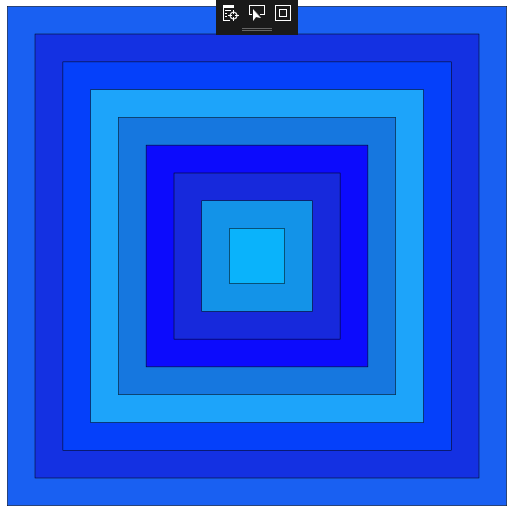
\includegraphics{square_boxes_res.png}
\end{figure}

\subsection{9 kwadratowych pudełek}
Dane wejściowe: 9 różnych kwadratowych pudełek, o wymiarach od 1x1 do 9x9 (podanych w losowej kolejności). 
Wynik: Lista zawierająca wszystkie pudełka.


\section{Wnioski}

\section{Podział pracy}


\end{document}